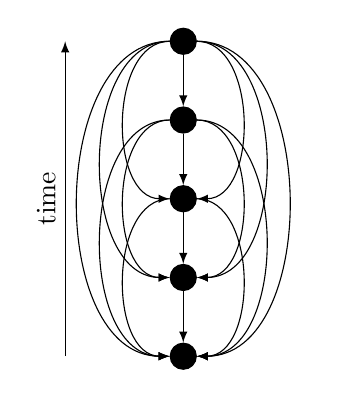
\begin{tikzpicture}
  \tikzstyle{bDot}=[circle, fill=black, draw]
  \foreach \y in {1,...,5} {
    \node[bDot] (D-\y) at (0, \y) {};
  }

  \foreach \y in {1,...,4} {
    \pgfmathsetmacro{\z}{int(\y + 1)}
    \draw[-latex] (D-\z) -- ({D-\y});
  }

  \foreach \y in {1,...,3} {
    \pgfmathsetmacro{\z}{int(\y + 2)}
    \foreach \j in {\z,...,5} {
      \ifthenelse{\y=2 \OR \y=3}{
        \draw[-latex] (D-\j) to[bend right=90] (D-\y);
      }{
        \draw[-latex] (D-\j) to[bend left=90] (D-\y);
      }
    }
  }

  \draw[-latex] (-1.5, 1) -- (-1.5, 5) node[midway, above, sloped]{time};
\end{tikzpicture}
